Alle Komponenten der Applikation werden in jeweils einem Docker Container ausgeführt, um unabhängig vom Betriebssystem oder installierter Software (bis auf Docker) zu funktionieren. 
Damit die Container auch miteinander kommunizieren können, wurde im "docker-compose.yml" File ein Netzwerk namens "leoturnier" erstellt.

Das Frontend und Backend werden als Docker Image von einem Workflow auf Github Packages gepusht, welcher jedes Mal ausgeführt wird, wenn eine Änderung der Applikation auf Github gepusht wird.
Die Docker Images werden mit "Dockerfiles" gebaut. 

\section{Backend}

Das Dockerfile, das für das Docker Image des Backends benutzt wird, wurde von Quarkus automatisch generiert und sieht folgendermaßen aus. 

\begin{figure}[H]
    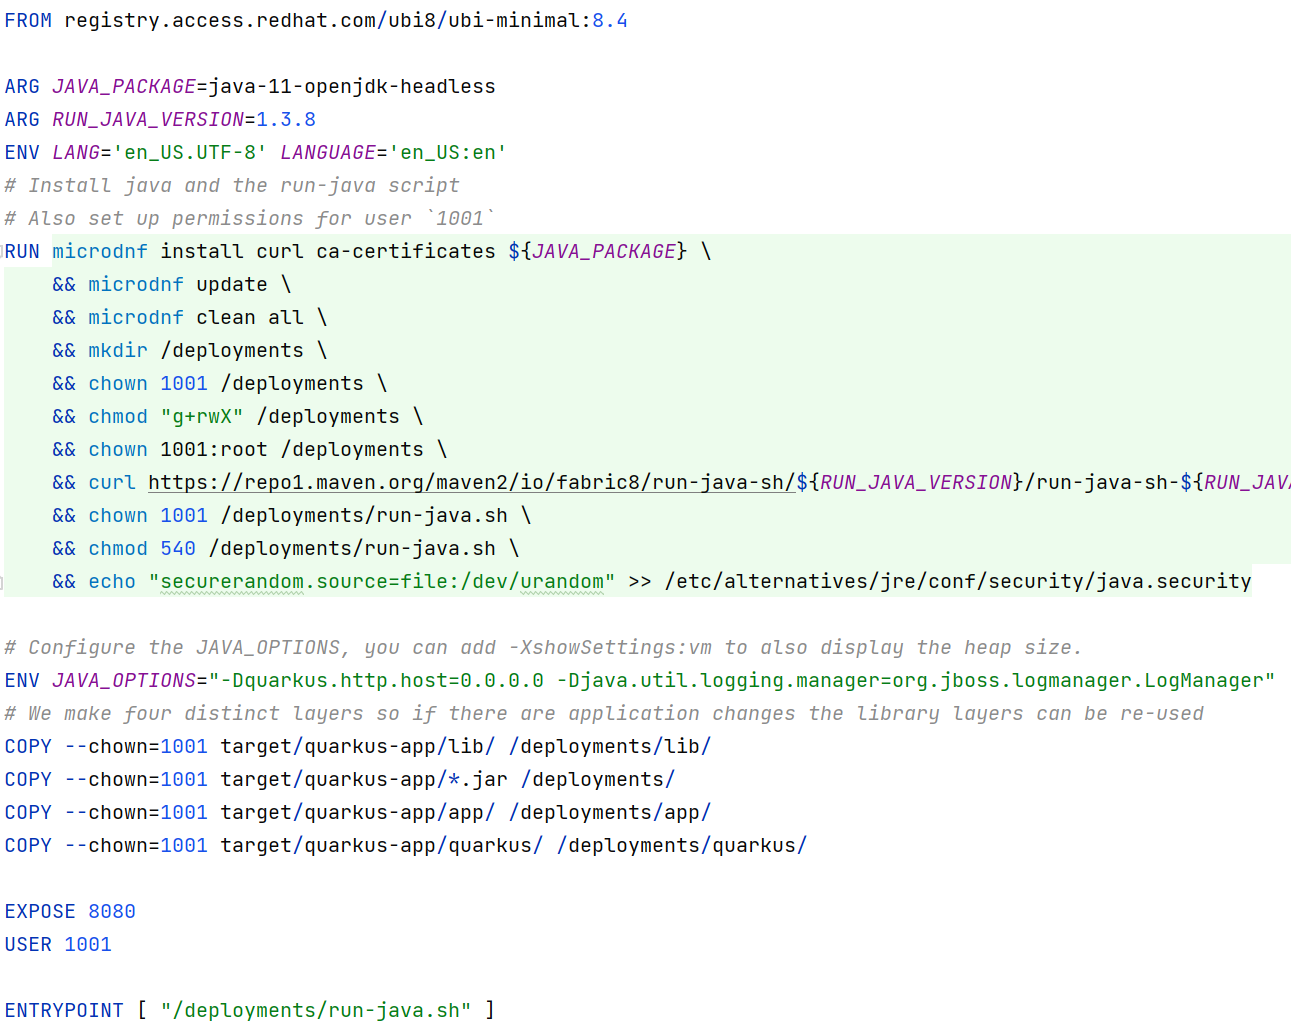
\includegraphics[scale=0.44]{pics/docker/dockerfile_backend.png}
    \caption{Dockerfile Backend}
\end{figure}

Im Grunde wird hier nur Java installiert und die für die Applikation wichtigen Files und Directories aus dem Backend in das Image kopiert.

Im Workflow wird dann die Registry angegebenen, in die das Image gepusht werden soll, in dem Fall Github Packages, anschließend wird das Image gebaut und dann gepusht.

\begin{figure}[H]
    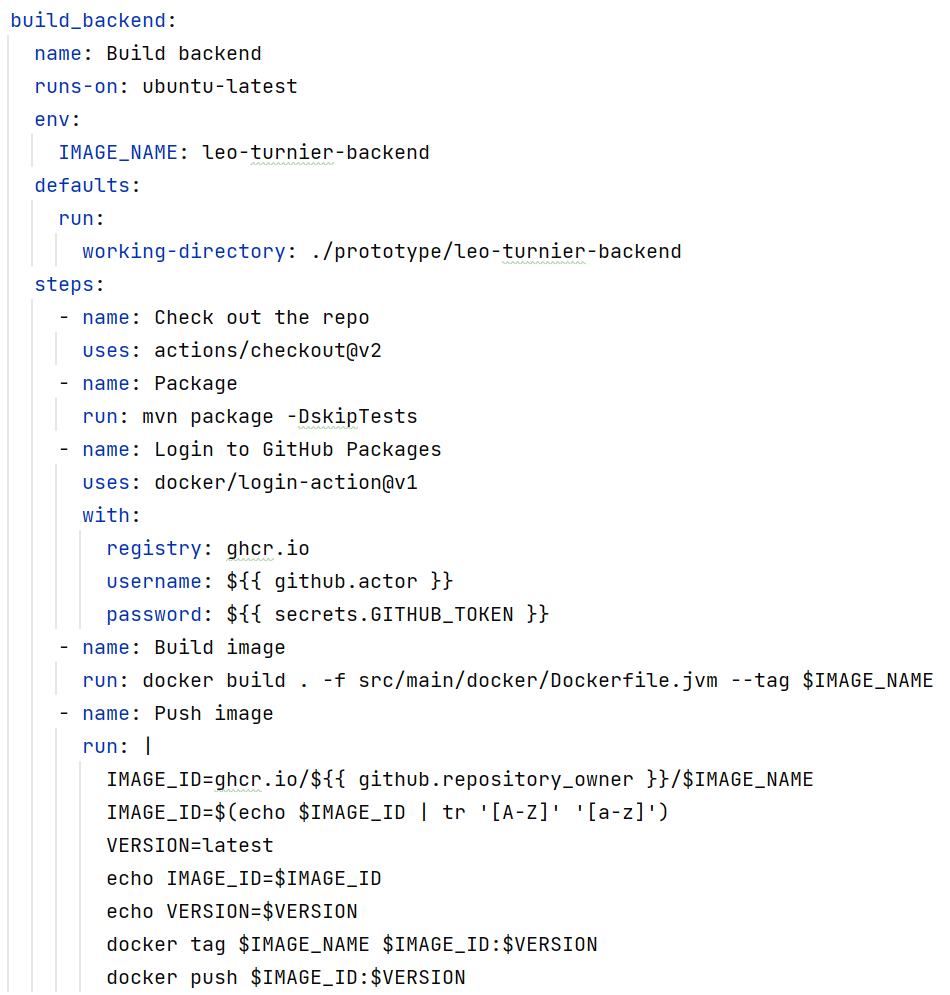
\includegraphics[scale=0.4]{pics/docker/workflow_backend.png}
    \caption{Workflow Backend}
\end{figure}

Ausgeführt wird das Image dann in einem Docker Container, der im dem "docker-compose.yml" File gestartet wird. 

\begin{figure}[H]
    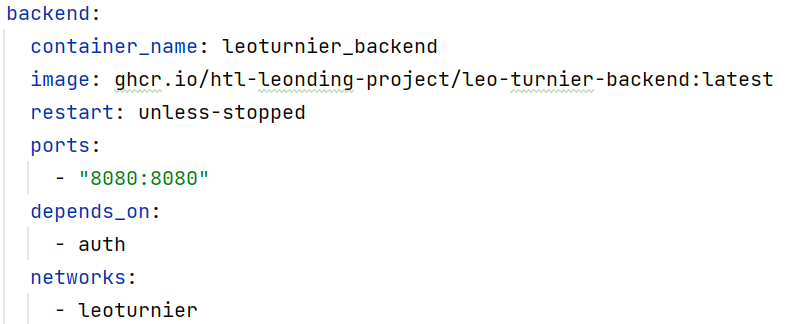
\includegraphics[scale=0.4]{pics/docker/docker-compose_backend.png}
    \caption{Docker Compose Backend}
\end{figure}

Hier wird das Docker Image, das im Vorhinein vom Workflow gepusht wurde, heruntergeladen und mit dem Port 8080 gestartet.

Zuvor wird noch die PostgreSQL Datenbank, in der die Turnierdaten gespeichert werden, gestartet.

\begin{figure}[H]
    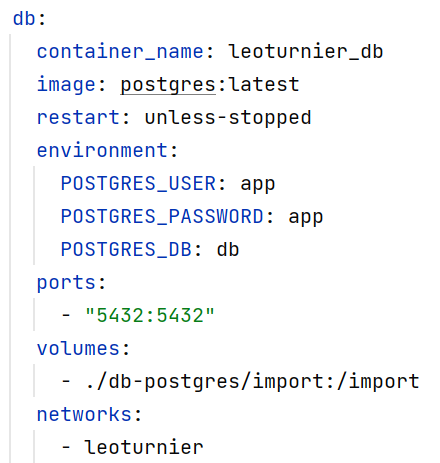
\includegraphics[scale=0.4]{pics/docker/docker-compose_db.png}
    \caption{Docker Compose Datenbank}
\end{figure}

\section{Frontend}
\setauthor{Benjamin Ecker}

\section{KeyCloak}

Der KeyCloak Server sowie die Datenbank, in der die Userdaten verwaltet werden, werden ebenfalls im "docker-compose.yml" File gestartet.

\begin{figure}[H]
    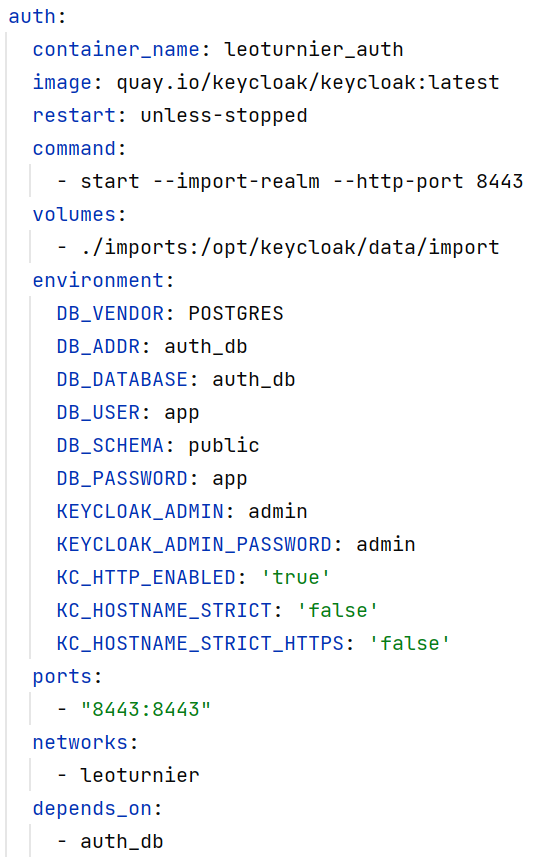
\includegraphics[scale=0.4]{pics/docker/docker-compose_auth.png}
    \caption{Docker Compose KeyCloak}
\end{figure}

Es werden die Konfigurationen importiert, der Port festgelegt, und User und Passwort für die verwendete Datenbank angegeben, welche zuvor ebenfalls im "docker-compose.yml" File gestartet wurde.

\begin{figure}[H]
    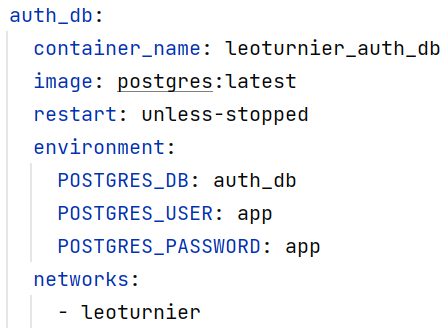
\includegraphics[scale=0.4]{pics/docker/docker-compose_auth_db.png}
    \caption{Docker Compose Userdatenbank}
\end{figure}